% This is the atech.tex This is where your writ ting will actually occur. In addition you will use this to display pictures, make tables, and format your paper. You should ONLY change things in this document.

% Calls up multiple packages that tell the computer ow you want to format the text and what neat tools you want to include so that you can use.

\documentclass[12pt]{article}
\usepackage{fancyhdr}
\usepackage{lettrine}
\usepackage[english]{babel}
\usepackage{graphicx}
\usepackage{gensymb}
\usepackage{listings}
\usepackage{multicol}
\usepackage{amsmath}
\usepackage{fancyvrb}
\usepackage{verbatim}
\usepackage{float}
\usepackage{multirow}
\usepackage{mathdesign}
\usepackage{txfonts}
\usepackage{mathrsfs}
\usepackage[justification=centering]{caption}
\usepackage{subcaption}
\usepackage{mdsymbol}
\usepackage{wrapfig}
\makeatletter
\def\mycatheader#1{\multicolumn{\tabu@nbcols}{c}{#1}}
\makeatother
\pagestyle{fancy}
\usepackage{mcode}
\providecommand{\e}[1]{\ensuremath{\times 10^{#1}}}

% Your class and semester here!
\lfoot{ECEN 1400}
\rfoot{Fall 2023}
 
% Defines that all Images are in the folder "images/" so that we don't have to type it repeatedly
\graphicspath{ {images/} }

% Catchy Name of your Project followed by 
\title{Atech Proposal: your project name}
%  followed by 
% Names {First Last} in Alphabetical Order by Last Name Go in Here 
\author{
  Name One \footnote{email1},
  Name Two \footnote{email2},
  Name Three \footnote{email3},
  Name Four \footnote{email4}\\
    {\normalsize 
   Lecture Section 100, ECEN 1400}\\
 }

% Tells the Document you are ready to start typing
\begin{document}

% Explains to the document to put in the Title, Names  onto a cover page
\maketitle

% This should be an ~200 word summary of the proposal
\begin{abstract}
An abstract is a block of text at the beginning of the paper that is usually around 200 words long. It is a conclusive statement of your entire proposal. 
\end{abstract}

% This ends the Title and Abstract page and lets you move on to the real report!

%This makes a new page 
\newpage

% This will make a Table of contents that Updates Automatically!
\tableofcontents

% This ensures it stays on its own page -- please be sure to do a new page before each new section (not subsection)
\newpage

% Begin a New Overarching topic
\section{Inspiration}
\newpage

\section{Project Scope}
The \textbf{scope} of the project will help you define the effort required and your plan to meet the specifications. This will help you figure out if the project is \textit{right sized} for the time you have. This judgement will depend on your skills - one size does not fit all.
% Begin a Sub-Topic
\subsection{Goals}
The goal and mission of your group should be in here. In addition pertinent information regarding your client (if you have one) will be very important. You should be explaining who they are before you explain what they need you to do! Be \textbf{very} descriptive.  What are your goals for the project? What is important for you to get out of it? These could be learning goals or specific performance milestones. (not the dates of PDR, CDR etc but what will be done) 

\subsection{Team Assignments}
Each should include a short description of what each person will do, sufficient to judge the effort and complexity of their task. What background, if any, does the team member bring that is relevant to achieving their goal? Everyone must do some technical design work – not just paperwork. Though certain students may have a larger or smaller technical role.

\subsection{Plans to Achieve Goal}
Depending on the project, describe:
\begin{itemize}

\item What will you design and build vs. what will you buy? (Buying pieces to help the design work is acceptable for this project)

\item What resources are available (people, existing designs) that increase your capability?

\item What will your project NOT do?

\end{itemize}

\newpage

\section{Specifications}

To the best of your ability now, list quantifiable performance specifications. Be as complete as you can. It is much more important that you think of the entry, (e.g. “Battery Life in Hours”) than you know the value.

% have text introducing the table

\begin{itemize}

    \item Start with categories, then work on individual entries.

    \item Present this in the form of a table. For each spec, list minimum, nominal and maximum values if known, \textit{as appropriate}. Include a column for units.

\end{itemize}
%Google "latex table format" 

\newpage

\section{Design Iteration}

% Sub-Topic 1
\subsection{Design Elements}
% each as appropriate for your project
This should be a full length description of your initial ideas/parts with beautiful pictures to match. I have elected to leave in a groups photo of their project to show how to insert a graphic below!

% This is how you insert a graphic. This is very, very important. Have this ready to go at all points. Always caption and use a label with your figure. Always reference the figure before you insert it.

% How to call a figure that has been labeled so you don't have to keep track of numbers.

Figure \ref{fig:frame} shows a rendering of our project frame including (be descriptive) a clear object in the front and the mounting system.

\begin{figure}[H]
% Puts your image in the center of the page, multiple other justifications are able to be done
\centering
    % Actually include the graphic
    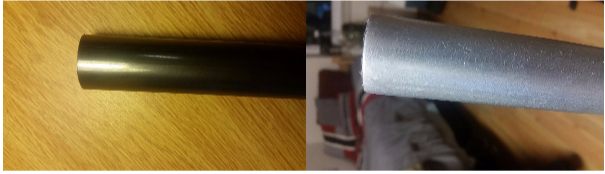
\includegraphics[width=6cm,height=4cm]{figure4}
    % CAPTIONS ARE VERY IMPORTANT NO FLOATING PICTURES
    \caption{Comparison of galvanized metal (right) to weldable steel (left)}
    % This is how we can tell the code what picture we are referencing.
    \label{fig:frame}
\end{figure}




\begin{itemize}
\item Block Diagram Electrical
\item Software Flow Chart
\item Block Diagram Mechanical
\item Sketch of package / external design - hand drawings are acceptable (if done in dark ink and readable - but preliminary CAD is encouraged. This should include how major components (in size or importance) are expected to “fit” in the project.
\item \textbf{Estimated}  bill of materials (BOM) as a \textbf{table} including cost for critical and expensive items. Total the cost. 
\end{itemize}

% Please use numbers/equations

In case you were wondering, you can use equations! See Equation \ref{eq:Strain}. This one happens to represent strain on a bar.

% This is how to use an equation, a mathematical Symbol, Fractions, and underscores
\begin{equation}
    \sigma = \frac{F}{A_{0}}
    \label{eq:Strain}
\end{equation}

% New Topic
\newpage
\section{Risk Mitigations}
\begin{itemize}
    \item List possible (significant) risks to success and briefly describe your plan to overcome these. Suggest minimal performance and alternative approaches or alternative goals to be successful. (think safety, supply chain issues, illness of team member, etc..)
    \item Think creatively about this.
\end{itemize}

% Another Figure example
In Figure \ref{fig:cage} you can see an old picture of the cage. 
\begin{figure}[H]
\centering
    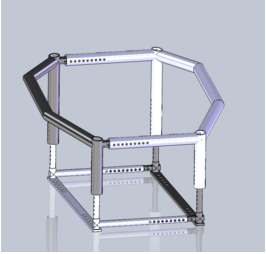
\includegraphics[width=12cm,height=8cm]{figure2}
    \caption{Original 3D model of the cage}
    \label{fig:cage}
\end{figure}

\newpage
\section{Timeline}
% New Sub-Topic
Look at the semester schedule including assignment milestones. Create a list of performance milestones by date. (what will get done by when) Include deliverables on sub-tasks such as electronics or software.  Use a \textbf{Gantt Chart} made using excel or something like excel.  Avoid using commercial packages or templates to create the chart, especially those that are complicated.

\newpage
\section{Tools}
Tools that will be used (laser cutter, 3D printer, sewing machines, milling machine). 
Put in any other tools you might have used!

\newpage
\section{Anything else you can think of that is helpful}

\newpage
\section{Closing Statements}
A strong argument for the success of this project
 
\newpage

% Anything Pertinent but without a real place, or if it doesn't fit in your discussion section.
\section{Appendix}

% Close and render the paper to a PDF format
\end{document}